\section{Overview}

As robots enter human-centric environments, they must learn to act and achieve the intended goal based on natural language instructions from a human partner. The robot should be able to achieve this goal in different environments, with perceptual and lingual variation in environments and instructions it has seen before. We want to take a step towards building general robots which can be trained quickly in new environments, and can generalise well to complex instructions and scenes than what they have seen during training, necessitating them to have visuo-linguistic reasoning abilities. As the robots operate in novel environments without dependence on expert operators or users, they should learn with easily available data without fine-grained expert annotations.
%

We first address this problem of language-guided robot manipulation, which involves learning to translate high level language instructions into
executable programs grounded in the robot’s state and action space, and learning representations for visual and action concepts that can be composed to achieve the task.
%
We focus on multi-step manipulation tasks that involve object interactions such as stacking and assembling objects referred to by their attributes and spatial relations. 
%
We assume the presence of natural supervision from a human teacher in the form of input and output scenes, along with linguistic description for a high-level manipulation task. 
%
We also focus on making our approach interpretable, with an ability to reason and visualise the effects of actions before actually executing them.

We introduce a \textbf{neuro-symbolic approach} built on the concept learning framework by \cite{Mao2019NeuroSymbolic} for jointly learning representations for concepts that can be composed to form \emph{manipulation programs}: symbolic programs that explain how the world scene is likely to affected by the input instruction. The \emph{manipulation program} is grounded into the scene to get a sequence of actions that are fed to the low-level motion planner of the robot. 

For our study, we look at a table-top setting consisting of blocks of various types and colours, with instructions like \emph{"put the block which is behind the green dice to the right of the red cube"}, as can be seen in figure \ref{fig:example-nsrm}. The goal is to produce a high-level task plan consisting of a sequence of \textit{sub-goals} which a robot manipulator can execute, where each sub-goal consists of the knowledge of the object to be picked (i.e. a pick location) and its target position (i.e. a place location).
%

\begin{figure}
    \centering    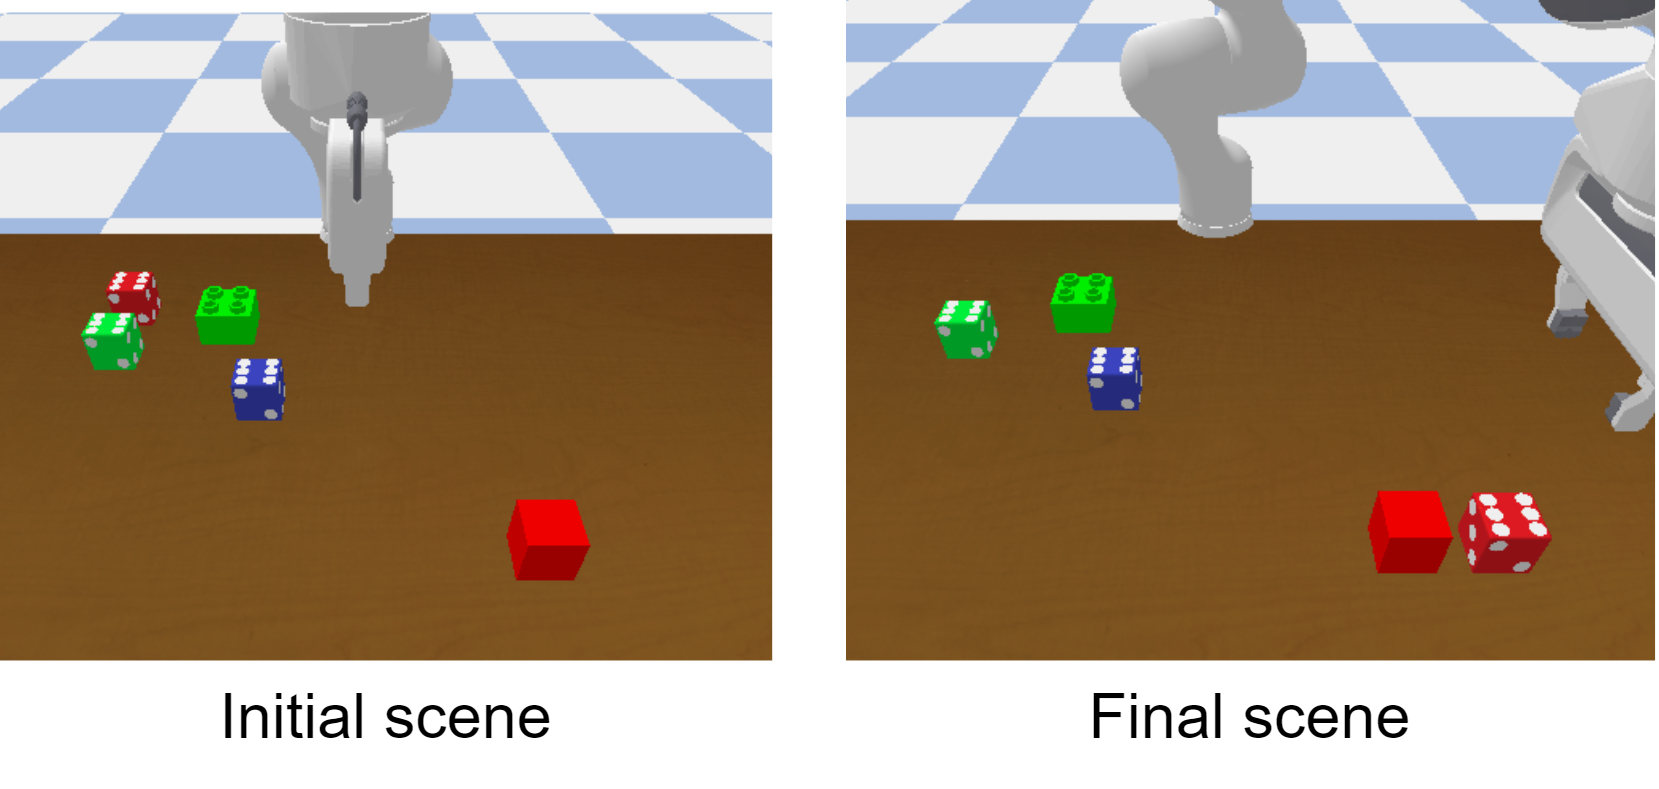
\includegraphics[width=0.6\textwidth]{assets/example-nsrm.png}
    \caption{An example from our dataset, with the natural language instruction \emph{"put the block which is behind the green dice to the right of the red cube"}}
    \label{fig:example-nsrm}
\end{figure}

While the generated plans may be perfect in simulation, there are often marred by imperfections in the real world caused by noise in the sensory inputs, motor failures, or unexpected collisions. This results in deviations from the original path of planned execution, which the agent needs to recover from. An example can be seen in figure \ref{fig:error-example}, where the block falls off from the gripper mid-journey to the next sub goal. 

\begin{figure}
    \centering
    \begin{minipage}{0.3\textwidth}
\includegraphics[trim={6cm 9cm 6cm 0},clip,width=0.9\textwidth]{assets/error-0.jpg}
    \end{minipage}
\begin{minipage}{0.3\textwidth}        \includegraphics[trim={6cm 9cm 6cm 0},clip,width=0.9\textwidth]{assets/error-2.jpg}
    \end{minipage}
\begin{minipage}{0.3\textwidth}        \includegraphics[trim={6cm 9cm 6cm 0},clip,width=0.9\textwidth]{assets/error-3.jpg}
    \end{minipage}
    \caption{Example of an execution error, due to a block falling off from the gripper. The original instruction was \emph{"put the white cube on top of the pink cube"}}.
    \label{fig:error-example}
\end{figure}

Often, the considerations of efficiency both in terms of time it takes to recover from the error, in terms of re-planning, as well as the time it takes for the new plan to reach the goal state, both become important. Further, even before recovery can happen, it is imperative that failures be correctly detected. We also note that this problem should be dealt without relying on hand annotated failure datasets, as they may be both time-consuming and expensive in terms of the human effort involved.  
%

Hence, our second goal is to build a scalable, self-supervised error detection and recovery mechanism which is efficiently able to detect discrepancies and reach the original goal while minimizing the time taken to re-plan. For our study, we simulate failures consisting of random external forces and perturbations of objects. We experiment with both single as well as multiple failures in a given plan. We introduce an efficient approach for \textbf{discrepancy-aware} failure-recovery mechanism based on an neuro-symbolic object-centric state representation.


\section{Problem Definition}

We thus address two problems in robot manipulation and task planning:

\textbf{Problem 1 [Learning Manipulation Programs]}: Given an initial world state and a natural language instruction, determine a sequence of sub-goals, which result in the final world state conforming to the instruction's intention.

The initial world state is given in the form of an RGBD image, and each sub-goal consists of the knowledge of the object to be manipulated and its target position. Only the final world state (as an RGBD image) is available for supervision during training. A DSL (Domain Specific Language) consisting of concept symbols is known, however their semantics are unknown. It is desired to achieve generalisation to novel scenes, instructions and plan lengths beyond those encountered during training, along with interpretability in sub-goals.

\textbf{Problem 2 [Error Detection and Recovery]}: For a robot manipulator executing a given plan on an initial world state, at each intermediate state, (i) determine if an error has occurred, and (ii) synthesise a plan to recover from the error so that the goal can be reached

For this problem, no addditional training data is assumed other than the data for the previous problem, specifically, no separate failure dataset is available for supervision. It is desired that the error recovery is quick, with minimal time taken for re-planning.

\section{Motivation}

The first problem of learning manipulation programs is hard since
\begin{enumerate}
    \item object attributes and actions have to be parsed from the underlying natural language sentence
    \item object references need to be grounded given the initial image.
    \item the effect of executing the specified actions has to be deciphered in the image space, requiring complex natural language as well as image level reasoning.
    \item The model needs to be trained end-to-end, learning representations for concepts via distant supervision.
    \item The approach needs to be interpretable and achieve generalisation to novel scenes and instructions
\end{enumerate}

Prior efforts for this problem can be broadly categorized as 
\begin{enumerate}
    \item Traditional methods which learn a mapping between phrases in the natural language to symbols representing robot state and actions in a pre-annotated dataset~\cite{howard2014natural,paul2016efficient,tellex2011approaching,matuszek2013learning,knepper2013ikeabot,gopalan2018sequence,williams2018learning}. They lack the flexibility to learn the semantics of concepts and actions on their own, which is an important aspect required for generalizability.
    \item Approaches that model an instruction as a sequence of action labels to be executed, without any deeper semantics, and requiring intermediate supervision for sub-goals, which may not be always be available~\cite{paxton2019prospection,shah2018bayesian,wang2020learning,kress2008translating,lazaro2019beyond,tenorth2010understanding,lisca2015towards,misra2016tell} 
    \item Recent end-to-end learning approaches~\cite{konidaris2018skills,wang2021learning, zettlemoyer2005learning,xia2018learning,silver2020few,zhu2021hierarchical,shridhar2022cliport,zeng2020transporter}; they have limited reasoning capability both at the level of instruction parsing, and their ability to learn varied action semantics.
\end{enumerate}

In response, our neuro-symbolic approach addresses these issues
\begin{enumerate}
    \item Our approach makes use of a Domain Specific Language (DSL) which specifies various concepts whose semantics are learned by the model. This allows generalizability to linguistic and perceptual variations in instructions and scenes respectively.
    \item The model is trained end-to-end and requires no intermediate sub-goal supervision. This allows training on easily obtainable form of data.
    \item Our latent neural object-centric representation allows for deeper reasoning needed to handle complex instructions and actions
\end{enumerate}
%

Prior works for the second problem on error recovery have been as follows

\begin{enumerate}
    \item Classical works have examined this problem in a purely symbolic setting, where the discovery simply corresponds to a goal check function, and recovery assumes the form of re-planning to the original goal, or repair to the sub-goal of last deviation from the plan.
    \item Alternate RL-based approaches learn a reactive policy that yield a high likelihood of reaching the goal from any state. However, they rely on well-enough offline exploration of the state space which is often difficult in complex manipulation domains.
    \item  More recently, literature has examined models which deal with perceptual data, containing various kind of noise, resulting in corresponding models for error recovery which account for variations in the input. Most approaches require hand annotated data sets, to learn a supervised function for discriminating two states from each other, both for error recovery, as well as re-planning. Creating such annotations, especially for failures, may be both time-consuming and expensive, in terms of the human effort involved. 
\end{enumerate}

%
In our work, we take a different approach to this problem, and ask the following question "Is there a way to learn a state discriminator function in a self-supervised manner which does not required hand annotated data for failed states?". An affirmative answer to this question would presumably help in building a scalable error recovery mechanism. Further, even after the failure has been detected, we would like to be efficiently able to reach the original goal while minimizing the time taken to re-plan, which can be prohibitive~\cite{fox2006plan}. This requires doing an efficient plan search to the desired sub-goal, which can exploit the localised information about where the failure might have occurred. 

Motivated by these questions, we propose an efficient approach for discrepancy aware failure recovery mechanism based on an object-centric scene-graph based state representation. 

\begin{itemize}
    \item Our state representation is decomposed in terms of individual object representations, which enables the agent to quickly discover what part of the state need to be changed to achieve the desired sub-goal, which is often the last state with correct execution of the original plan. 
    \item Central to our approach is a set of neural discriminators to separate out two different state as well as object representations trained in a self-supervised manner. Our discriminator not only detects failure, but also provides localised information about which objects have caused the failure by discriminating object representations.
    \item The search for recovery plan to the sub-goal, which is the last correct state, focuses on those objects which are the cause of the error as per the information provided by discriminator and manipulate these objects ignoring others. This results in a forward search accelerated with learned heuristics operating on a neuro-symbolic domain representation.
\end{itemize}


\section{Contributions}

For the first problem, our contributions are: 
%
\begin{enumerate}
\item A novel neuro-symbolic model that learns to perform complex object manipulation tasks requiring reasoning over scenes for a given natural language instruction and given initial world scene, without intermediate supervision.  
%
\item A CLEVR-like dataset for language-guided robot manipulation, consisting of a table top setting with a 7-DOF manipulator, blocks of various shapes and types, and language instructions with various levels of complexity.
%
\item Ability to interpret and visualise the model's latent program space by reconstructing any intermediate scene before execution by the manipulator 
%
\item Evaluation in instruction following experiments with a simulated robot manipulator, demonstrating robust generalization to novel settings improving on the state-of-the-art.
\end{enumerate}

This work is discussed in detail in chapter \ref{chap:part-1}. It was accepted at the International Conference on Robotics and Automation 2023 (\url{https://www.icra2023.org/}) as \\
\textbf{Learning Neuro-symbolic Programs for Language Guided
Robot Manipulation} \\
Namasivayam K$^{*}$, Himanshu Singh$^{*}$, \emph{Vishal Bindal$^{*}$}, Arnav Tuli, Vishwajeet Agrawal, Rahul Jain, Parag Singla, Rohan Paul

Information regarding the paper, video and code is at \url{https://nsrmp.github.io/} 


 For the second problem, our contributions are:
 \begin{enumerate}
     \item An efficient approach for discrepancy-aware failure detection and recovery, based on a neuro-symbolic state representation
     \item Neural modules for state transition and discrimination learned without any additional failure datasets
     \item A recovery mechanism consisting of forward search guided with learned heuristics
     \item Evaluation with various degrees of simulated errors, demonstrating strong improvement over baselines in terms of time taken for error recovery
 \end{enumerate}

 This work is discussed in detail in chapter \ref{chap:part-2}. It is currently under review at Conference on Robot Learning 2023 (\url{https://www.corl2023.org/}) as \\
 \textbf{Learning to Recover from Plan Failures using Fast Discrepancy-Aware Neuro-Symbolic Search} \\
 Arnav Tuli$^{*}$, \emph{Vishal Bindal$^{*}$}, Namasivayam K, Himanshu Singh, Parag Singla, Rohan Paul
